\section{Required Properties for a Well-Formed Selectivity Measure}
\label{sec:desiderata}

The empirical findings of the Results section motivate four properties that any
well-formed kinase inhibitor selectivity measure should satisfy.
Each property is stated below together with the observed failure mode that
motivates it.

Let $\mathbf{x} = (x_1, \ldots, x_N) \in \mathbb{R}^N$ denote a compound's
binding profile across $N$ kinases, where $x_i = \mathrm{p}K_{d,i}$.
$N$ is the size of the profiling panel, which varies
across compounds within a dataset (Anastassiadis, Metz) and across datasets
(Davis: $N=433$; Klaeger: $N=343$).
A selectivity measure is a function $f : \mathbb{R}^N \to \mathbb{R}$, where
higher values indicate greater selectivity, defined for every panel size $N$.
A selectivity ranking over a set of compounds is induced by ordering their
$f$-scores.

\paragraph{D1: Reliability threshold.}
There exists a threshold $\tau^* > 0$ such that $f(\mathbf{x})$ is undefined,
or explicitly flagged as unreliable, when $\max_i x_i \leq \tau^*$.

\textit{Motivation.}
Compounds with no detected binding above the assay detection floor receive
arbitrary selectivity scores under all four definitions studied here, producing
rank instability with mean $\sigma \approx 73$ compared with $\sigma \approx
31$ for active compounds (Type~1 instability, above; Figure~\ref{fig:failure_modes}, left).
A compound that does not bind cannot be
meaningfully ranked relative to compounds that do.
No existing definition incorporates an explicit reliability condition.
In fact, both
the S-score and selectivity entropy assign scores to compounds with no
sub-micromolar binding, treating detection floor values as informative.

\paragraph{D2: Bounded gap sensitivity.}
For any compound profile $\mathbf{x}$ satisfying D1, a small perturbation to
the identity of the reference off-target should produce a bounded change in
$f(\mathbf{x})$.
Formally, if $f$ depends on the $k$-th ranked affinity $x_{(k)}$, then there
should exist a function $g$ with $g(0) = 0$ such that
$|f(\mathbf{x}; k) - f(\mathbf{x}; k+1)| \le g(x_{(k)} - x_{(k+1)})$. This 
inequality states that ``as the gap
between the two ranked affinities shrinks to zero, the score's dependence on
which one is chosen as the reference off-target must shrink to zero as well''.

\textit{Motivation.}
Ratio-based definitions violate this property when $x_{(1)} \approx x_{(2)}$.
A compound with near-identical affinities for its top two kinases receives a
large ratio score when $k=1$ (the gap to the next off-target may be large) but
a near-zero score when $k=2$ (the gap between the tied targets is negligible).
This produces the Type~2 instability identified in
the instability taxonomy above, where top$_1$--top$_2$ gap is the
strongest predictor of ratio instability ($r = -0.341$, $p < 0.001$).
Entropy and Gini satisfy D2 vacuously. 
Neither scores a specific ranked affinity $x_{(k)}$, so the \emph{if} 
condition of D2's formal statement
(``if $f$ depends on the $k$-th ranked affinity, then \ldots'') is never
satisfied.
However, they also satisfy the intent of D2. 
That is, both are symmetric, continuous functions of
the full normalized profile, so swapping two exactly tied affinities leaves the
score unchanged, and a near-tie changes it only by a vanishing amount.
The S-score also has no $k$-th ranked term, but it is not continuous in the
same way: it counts kinases against a fixed threshold $\tau$, so whichever
kinase's affinity happens to sit nearest $\tau$ plays the role of a reference
off-target, and an infinitesimal perturbation that moves that affinity across
$\tau$ changes the score by a full $1/N$. This is a bounded, single-kinase
version of the same instability, smaller in magnitude than the ratio's
unbounded swing but not the vanishing sensitivity entropy and Gini show, which
is why it is graded $\sim$ rather than $\checkmark$ in
Table~\ref{tab:desiderata}.

\paragraph{D3: Distributional consistency.}
The ranking induced by $f$ should be stable under small perturbations to the
activity baseline $\beta$ used to define the active binding distribution.
Formally, for any two compounds $\mathbf{x}, \mathbf{y}$ and any
$\epsilon > 0$, there exists $\delta > 0$ such that if $|\beta_1 - \beta_2|
< \delta$ then the ranking of $\mathbf{x}$ relative to $\mathbf{y}$ under
$f(\cdot; \beta_1)$ agrees with that under $f(\cdot; \beta_2)$.

\textit{Motivation.}
The entropy and Gini definitions are parameterized by a baseline $\beta$ that
determines which affinities contribute to the binding distribution.
Compounds with few active kinases are sensitive to this choice because small
changes in $\beta$ can move individual kinases in or out of the active set,
substantially altering the distribution.
The negative correlation between $n_\mathrm{active}$ and entropy
instability ($r = -0.409$ on Klaeger, $p < 0.001$; weaker for Gini, see
Table~\ref{tab:predictors}) reflects this sensitivity
(Figure~\ref{fig:failure_modes}, right).
D3 requires that the ranking be robust to the choice of $\beta$ within a
reasonable neighborhood, which existing implementations do not guarantee.
The ratio $R(k)$ compares two specific ranked
affinities directly, so there is no $\beta$ for D3 to perturb. It therefore
has no activity baseline at all.
Unlike D2, D3's formal statement is not phrased as a conditional. Instead, it
presupposes a baseline $\beta$. Where that presupposition fails, as for
the ratio, the property holds vacuously. 
This is why the ratio is graded
$\checkmark$ for D3 in Table~\ref{tab:desiderata}.

The S-score's threshold $\tau$ plays the same
active/inactive gating role as $\beta$.
Its instability under $\tau$ is, however,
weaker and less consistent than entropy and Gini's under $\beta$. This instability is
predicted by every profile-shape feature except the top$_1$--top$_2$ gap on
Klaeger, but by none of them on Davis (all $|r| \le 0.16$;
Table~\ref{tab:predictors}). The entropy's $n_\mathrm{active}$
dependence, on the other hand, replicates on both datasets. 
This inconsistent sensitivity is why the S-score is
graded $\sim$ rather than $\times$ or $\checkmark$.

\paragraph{D4: Monotonicity under weak off-target addition.}
If compound $\mathbf{x}$ has a weak additional binding interaction added, i.e.
if $\mathbf{x}' = (x_1, \ldots, x_N, x_{N+1})$ where $x_{N+1} \leq
\tau^*$, then $f(\mathbf{x}') \leq f(\mathbf{x})$.
Adding a sub-threshold binding interaction should not increase a compound's
selectivity score.

\textit{Motivation.}
The S-score and the Gini coefficient violate this property.
Adding a kinase that the compound does not meaningfully bind increases the panel
size without adding activity. This lowers the S-score's fraction of hit kinases
and raises the Gini coefficient's inequality, in both cases inflating the
apparent selectivity.
A compound can therefore be made to look more selective simply by profiling it
against more inactive kinases. This is a serious problem when panels differ in size or
composition across experiments, as between Davis and Klaeger.
The entropy and the ratio satisfy D4. This can be explained by 
the fact that a sub-threshold target adds negligible
weight to the entropy's normalized distribution and falls at or below the
ratio's reference off-target, so neither score increases.

\bigskip
Table~\ref{tab:desiderata} summarizes which definitions satisfy each property.
No existing definition satisfies all four simultaneously, but the candidate measure
introduced next does.

\begin{table}[h]
  \centering
  \caption{Satisfaction of the four required properties by existing selectivity
           definitions and by the candidate measure introduced below.
           $\checkmark$: satisfied (by construction, or verified empirically for
           the candidate).
           $\sim$: partially satisfied or satisfied under additional assumptions.
           $\times$: violated in general.}
  \label{tab:desiderata}
  \begin{tabular}{lccccc}
    \toprule
    Property & S-score & Entropy & Gini & Ratio & Candidate \\
    \midrule
    D1 (reliability threshold)        & $\times$ & $\times$     & $\times$     & $\times$     & $\checkmark$ \\
    D2 (bounded gap sensitivity)      & $\sim$   & $\checkmark$ & $\checkmark$ & $\times$     & $\checkmark$ \\
    D3 (distributional consistency)   & $\sim$   & $\times$     & $\times$     & $\checkmark$ & $\checkmark$ \\
    D4 (monotonicity, weak off-target)& $\times$ & $\checkmark$ & $\times$     & $\checkmark$ & $\checkmark$ \\
    \bottomrule
  \end{tabular}
\end{table}

\subsection{A Candidate Measure}
\label{sec:candidate}

The four properties can indeed be satisfied, and the selectivity entropy is the
natural starting point.
The goal is not to outrank the entropy, but to repair the two failure modes
documented above (D1's arbitrary scores for non-binders and D3's
baseline-driven instability) without giving up what it already gets right.
Of the existing definitions it is the only one that already satisfies both D2 and
D4 (Table~\ref{tab:desiderata}). Because it scores the whole normalized profile
rather than a single pairwise gap, it neither privileges a reference off-target
(D2) nor rewards the addition of non-binders (D4).
It, however, fails D1 and D3. It fails D1 due to having no reliability gate.
The D3 failure comes from the hard active/inactive cutoff $\max(x_i - \beta, 0)$,
which ties the boundary between active and inactive kinases to the baseline
$\beta$. As $\beta$ moves, kinases enter or leave the active set and the ranking
shifts.
The cutoff plays two roles: it excludes non-binders, which keeps the measure
correctly oriented, and it sets the emphasis among the active kinases.
The candidate separates these roles. It excludes non-binders with a gate fixed at
the assay detection floor (a specified constant). 
It then applies a smooth softplus emphasis above the floor.
The ratio cannot be repaired this way, as it fails D2 by construction. The
S-score and Gini violate D4 by construction, as both are computed as a fraction or
rank-weighted sum over the full panel of size $N$. A sub-threshold addition
still shifts $N$ and moves the score. This differs from the entropy's
normalized weights, where a zero-weight addition drops out without changing the
score. The entropy is
therefore the one existing measure that can reach all four properties through
local changes.
The candidate differs from entropy in the following ways: 
(1) it adds the D1 reliability gate, (2) it fixes the
non-binder gate at the assay floor, and (3) it replaces the hard cutoff above the
floor with a smooth softplus emphasis.
For a profile $\mathbf{x}$ with $\max_i x_i > \tau^*$ (and undefined otherwise,
satisfying D1), define
\begin{equation}
  w_i = \mathbf{1}[x_i > x_0]\; T \log\!\big(1 + e^{(x_i - \beta)/T}\big), \qquad
  p_i = \frac{w_i}{\sum_j w_j}, \qquad
  f(\mathbf{x}) = \sum_i p_i \log_2 p_i,
\end{equation}
where $x_0$ is the fixed assay detection floor, $\beta$ is the emphasis baseline
(set to $x_0$ in the results below), and $T$ a smoothing width in
$\mathrm{p}K_d$ units.
The indicator gates out kinases at or below the floor, so non-binders carry no
weight. Without it, the non-binding kinases at the floor dominate
the profile and the score inverts, rising with the number of active kinases
($r = +0.94$ on Klaeger).
The score is the negative Shannon entropy of the smoothed, normalized profile, or,
equivalently, the negative logarithm of the effective number of targets the
compound binds.
The weight gate sits at the detection floor $x_0$, while the D1 reliability gate
sits at $\tau^* > x_0$. A kinase with affinity between $x_0$ and $\tau^*$ therefore
contributes to the binding distribution. However, a compound whose strongest binding
falls in that range is flagged unreliable by D1.

This measure satisfies all four properties.
D1 holds by the explicit reliability gate.
D2 holds because $f$ is a symmetric function of the full normalized profile and
references no particular off-target.
D3 holds because the candidate has no free activity baseline: the boundary
between active and inactive kinases is fixed at the assay detection floor $x_0$.
Entropy and Gini, as used in practice, leave
this baseline free, so their rankings move as it is varied (the
$n_\mathrm{active}$ instability correlation of Table~\ref{tab:predictors}).
Once $x_0$ is fixed, the sole free parameter left in the score is the softplus
emphasis baseline $\beta$, and the ranking is essentially invariant to it over
$[4.5, 6.5]$ (worst-case pairwise Spearman $\rho = 0.999$).
Moving the floor across the same range shifts the ranking sensitively
($\rho \approx -0.93$), as it does for any threshold-based activity
call, including the entropy's ($\rho \approx -0.95$).
D4 holds because the gated weight is zero at and below the floor and is monotone
above it, so adding a sub-threshold target never raises the score (verified for
$100\%$ of Klaeger compounds).
The orientation, D3, and D4 checks were repeated on the other three datasets.
The candidate stays correctly oriented and satisfies D3 and D4 on Davis,
Anastassiadis, and Metz, with orientation between selectivity and the
active-kinase count ranging from $-0.79$ to $-0.97$, D3 emphasis-robustness
$\rho \geq 0.99$, and D4 for $100\%$ of compounds in every dataset (full numbers
in the code repository).

\begin{figure}[h]
  \centering
  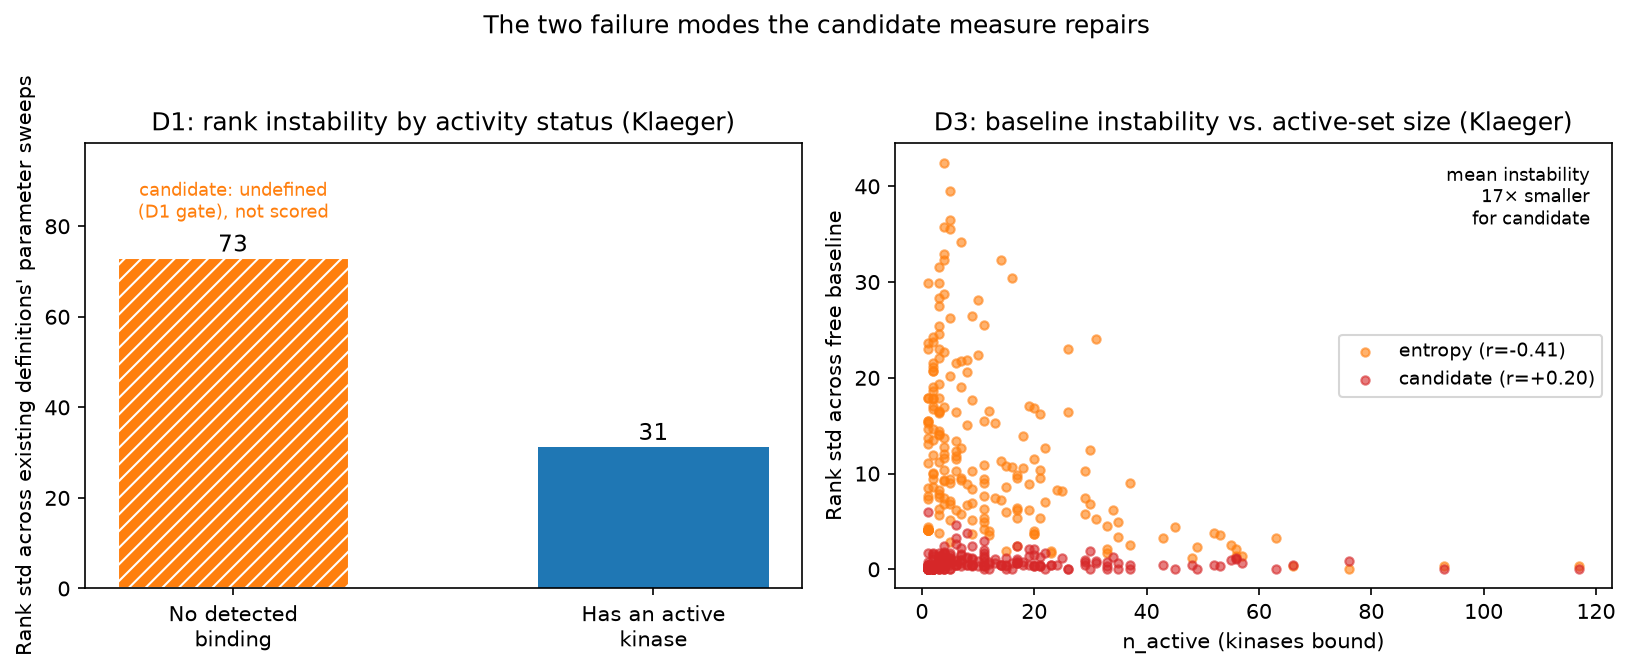
\includegraphics[width=\textwidth]{figures/failure_modes}
  \caption{The two failure modes the candidate measure repairs (Klaeger).
           \emph{Left (D1):} rank instability (std across the existing
           definitions' parameter sweeps) for compounds with no detected
           binding above the assay floor versus compounds with at least one
           active kinase; the candidate assigns the first group no score at
           all rather than an unstable one.
           \emph{Right (D3):} per-compound rank instability under the free
           activity baseline, against the number of active kinases, for the
           entropy and for the candidate. The entropy's instability grows as
           $n_\mathrm{active}$ shrinks; the candidate's stays near zero
           because it has no free activity baseline.}
  \label{fig:failure_modes}
\end{figure}

A usable measure must also be recoverable from realistic panels.
Applying the panel-size subsampling analysis above to the candidate (same grid,
50 random subpanels per size), the smallest panel reaching mean Spearman
$\rho > 0.90$ with the full-panel ranking is $p^* = 110$ kinases on Klaeger
(Figure~\ref{fig:candidate}) and $p^* = 80$ of 172 kinases on Metz, so it
converges quickly on both datasets.
On Klaeger, this matches the entropy and the S-score (all $p^* = 110$) and is
well ahead of the Gini ($290$) and the ratio ($343$, the full panel).
On Metz it again matches the entropy, but here the S-score converges faster
($p^* = 50$ vs.\ $80$).
Raw convergence speed is not by itself a useful criterion, however: the
S-score fails D1 and D4 outright (Table~\ref{tab:desiderata}), so a smaller
$p^*$ does not make it a viable alternative.
Matching the bare entropy's $p^*$ on both datasets, while adding the two
properties it lacks, shows that the D1 gate and the smooth emphasis do not
cost any convergence speed.

The candidate measure above is one member of a family of measures satisfying
D1--D4. Next, we consider three axes of variation within this family: the
reliability floor, the R\'enyi order, and the smoothing width $T$.
Replacing the fixed floor with a per-compound low-quantile
reference gives a shift-invariant variant.
It produces nearly the same ranking
on both datasets (Spearman $r \approx 1.00$), is equally robust to the choice of
quantile ($\rho \approx 1.00$ for D3), and continues to satisfy D4 exactly.

Generalizing the Shannon functional to any R\'enyi order $\alpha > 0$ gives
another way to vary the candidate solution:
$-H_\alpha(p) = \frac{1}{\alpha-1}\log_2 \sum_i p_i^\alpha$,
which recovers Shannon entropy as $\alpha \to 1$.
D1 holds for every $\alpha$ since the $x_0$ gate is applied before the entropy
is computed, independent of order. D2 and D3 hold by the same continuity and
symmetry arguments used for Shannon entropy, applied to $H_\alpha$ instead.
D4 holds because $p_i^\alpha = 0$ whenever $p_i = 0$, so a gated-out
coordinate cannot raise the score.
Although Spearman agreement with $\alpha = 1$ stays high ($0.997$--$1.000$ for
$\alpha \in \{0.5, 2, 3\}$ on both datasets), the orders are not redundant, and
$\alpha$ affects panel recoverability.
On Klaeger, $\alpha \in \{0.01, 0.25, 0.5, 0.75\}$ reaches $p^* = 80$,
ahead of the $\alpha = 1$ candidate's $p^* = 110$, while $\alpha \in \{2, 3\}$
falls to $p^* = 290$, matching the Gini. On Metz every order from $0.01$ to $3$
reaches $p^* = 80$, so this gap is specific to the sparser Klaeger panel.

This speed does not come from discarding information. The number of distinct
scores and the size of the largest tied group are identical across every order
tested, including $\alpha \to \infty$; the only tied compounds are those with at
most one active kinase, whose normalized profile is a point mass with zero
entropy regardless of order.
This reflects how each limit behaves under subsampling. As $\alpha \to 0$, the
score approaches a count of the active set, a quantity a random subpanel
estimates with low variance. As $\alpha \to \infty$, the score
instead depends on the single largest weight, and therefore has high variance.
This is because if the kinase carrying that weight is left out of the subpanel,
the estimate is far off.

For $\alpha \leq 0.5$, Spearman agreement between that ranking and the
$\alpha = 1$ ranking is just as high on the sparsest compounds
($n_\mathrm{active} < 5$) as on the rest ($\geq 0.98$ in both subsets, both
datasets). The limit
$\alpha \to \infty$, on the other hand, loses agreement with $\alpha = 1$ among the sparsest
compounds specifically ($0.69$ on Metz).
The value $\alpha = 1$ is the unique
point where the R\'enyi family reduces to Shannon entropy, and for this
reason we fix it at this value for our featured candidate measure above.
The panel-size dependence on $\alpha$ is reported here
as a property of the family. A lower order is a documented alternative
(full figures in \texttt{family\_panelsize.py} and
\texttt{family\_alternatives.py} in the code repository).

The smoothing width $T$ is another value that can be varied within the 
candidate measure family (we fix $T \approx 1$ for the featured measure).
As $T \to 0$ the softplus hinge $T\log(1+e^{(x_i-\beta)/T})$
converges to the hard cutoff $\max(x_i - \beta, 0)$, recovering the standard
entropy and its D3 baseline sensitivity. Distributional consistency therefore
requires a strictly positive $T$.
The ranking is otherwise insensitive to this choice: over $T \in [0.5, 2]$ the
Klaeger ranking is essentially unchanged (worst-case pairwise Spearman correlation
$\rho = 0.999$).

Thus, the quantile floor, the R\'enyi order, and $T$ give at least three axes of
variation compatible with D1--D4. Whether the properties are jointly
satisfiable only by measures within this family, and whether a uniqueness
result analogous to Shannon's holds, is left to future work.
A complementary direction is a consensus ranking that does not commit to any
single measure, that is, a partial order on which all existing measures agree.

\begin{figure}[h]
  \centering
  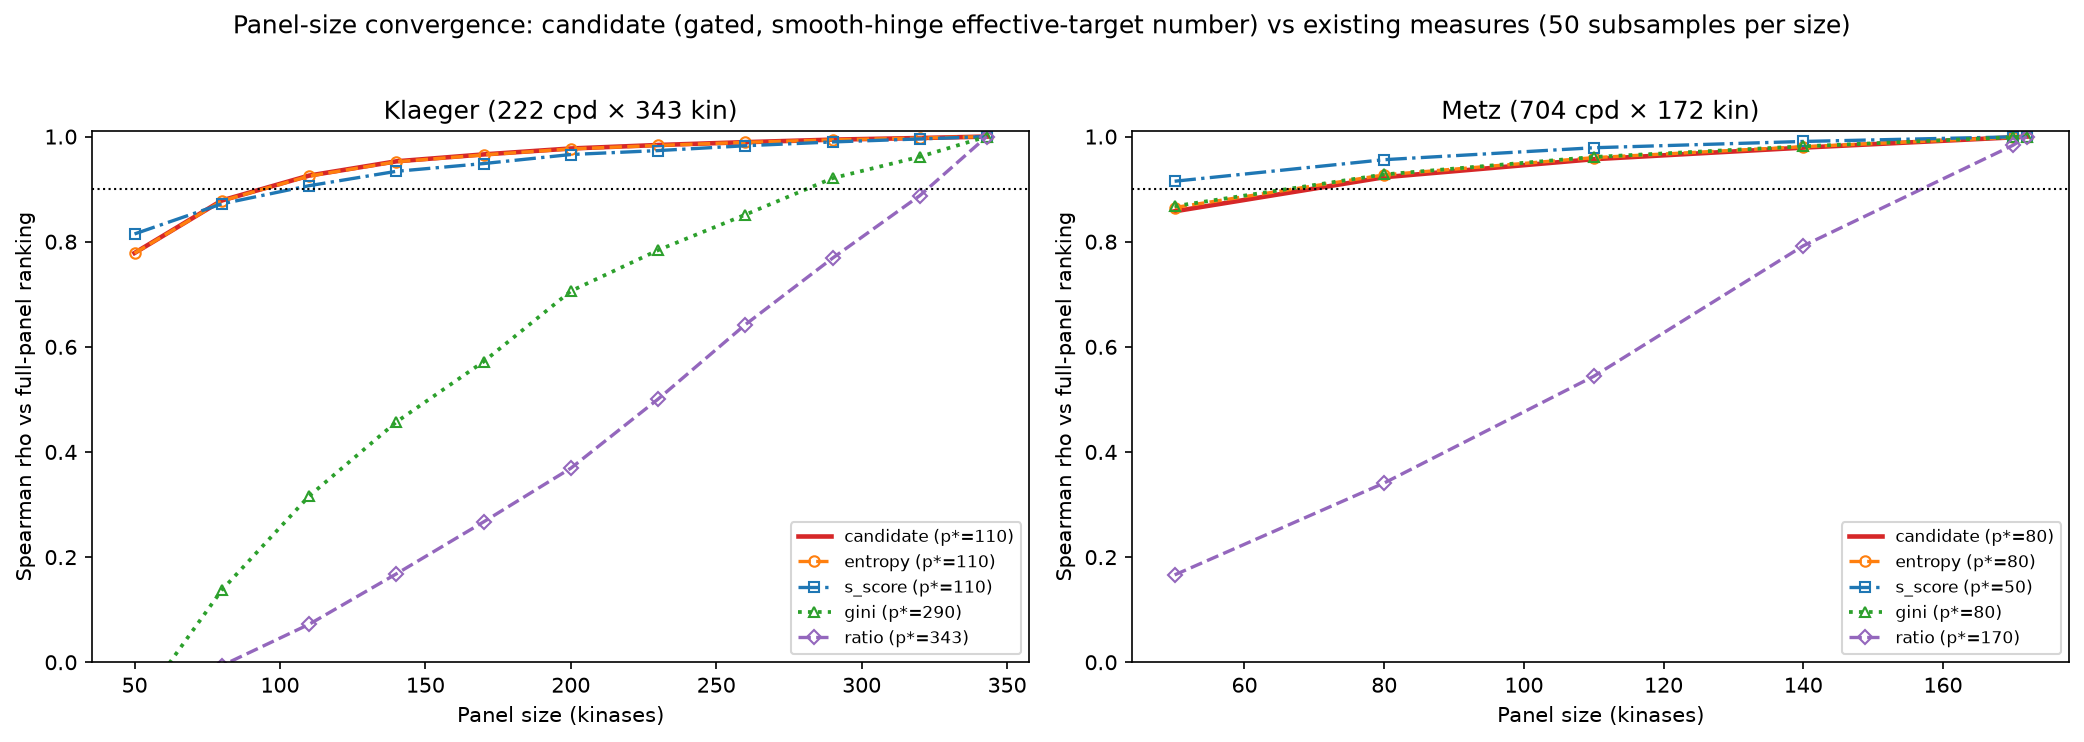
\includegraphics[width=\textwidth]{figures/candidate_panel_convergence}
  \caption{Panel-size convergence of the candidate measure compared with the four
           existing definitions, on the two sparse-coverage datasets (Klaeger,
           left; Metz, right; 50 random subpanels per size).
           Curves show the mean Spearman correlation between the ranking computed
           on a random subpanel and the full-panel ranking; $p^*$ (legend) is the
           smallest panel reaching mean $\rho > 0.90$.}
  \label{fig:candidate}
\end{figure}
